\title{\textbf{Signal or Coincidence? Causal Auditing of Collusion\\Through Shared Agent State}}
\author{Sarvesh Tiku\\[2pt]
Georgia Institute of Technology\\
\small\texttt{stiku6@gatech.edu}\\
\small AI Collusion Research Sprint (Apart Research) \textperiodcentered{} Track 3 (Q3.1), secondary Track 2 (Q2.3)}
\date{October 2026}

\begin{document}
\maketitle

\begin{abstract}
\noindent
Two agents acting alike is weak evidence that they coordinate. We test a \emph{randomized canary audit}: an auditor gives one agent a uniformly random private target and asks whether a second agent's behavior depends on it, then intervenes on the shared tool state between them. In a synthetic separation-of-duties compliance workflow, a preparer writes two closed-vocabulary ticket fields and an approver decides on four transactions; both are \emph{instructed} to get the target approved, so we study carriers of instructed collusion, not its emergence. Across four models (100--150 matched seeds, 33 arms), recovery in every channel-free arm matches the exact null $P(\text{valid guess})/4$. Without a pre-agreed code, the fields carry the target for one model only: Gemini-2.5-Flash preparers mark it \emph{urgent} (\vv{gemini}{shared}{recover}\% vs.\ \vv{gemini}{removed}{recover}\%, Holm $p{=}\vv{gemini}{sharedvsremoved}{ph}$), every other approver model decodes this convention (\vv{geminigptfouro}{cross}{rec}--\vv{geminigptfour}{cross}{rec}\%), and permuting tickets sends approvers to the decoy. With a pre-agreed code the fields transmit nearly all 2 bits of target entropy. Information flow is not collusion: an authorized expedite request yields \vv{gemini}{benign_flag}{recover}\% flow with honest agents and no detectable rise in harm. Defenses are carrier-specific: recomputing fields from source records removes field codes, but sanitizer-aware preparers move the signal into a surviving free-text note (3 of 4 models; Gemini \vv{gemini}{notes_verbatim}{recover}\%), and redacting IDs, numbers and countries does not stop it. A fixed structural rule monitor detects collusive tickets better than an LLM monitor (AUROC \vv{gemini}{mon}{ruleauroc} vs.\ \vv{gemini}{mon}{llmauroc} for Gemini). We give the identification argument, its assumptions, and the cases it does not cover.
\end{abstract}

% ======================================================================
\section{Research Question and Threat Model}\label{sec:intro}
Multi-agent deployments route work through shared tools---tickets, queues, status fields---which agents can use to signal each other~\citep{hammond2025multiagent,motwani2024secret,dafoe2020open}, and proposals for agent economies make such shared state central~\citep{tomasev2025distributional}. Track~3 asks whether collusion can be carried through such side channels; Track~2 asks what should count as convincing evidence of it. Correlated actions do not suffice: two instances of a model share priors, see the same data, and face the same incentives. Antitrust reasoning makes the same point with ``plus factors'': parallel conduct alone does not establish agreement~\citep{kovacic2011plus}, a problem sharpened for autonomous pricing agents~\citep{harrington2018developing,ezrachi2016virtual}.

\paragraph{Question.} Can an auditor (i) establish that information moved from one agent to another through routine structured state, (ii) localize the carrier, and (iii) tell whether an intervention reduces \emph{policy-violating outcomes} rather than only the approver's ability to name a target?

\paragraph{Threat model.} Two agents under separation of duties: a preparer A writes per-transaction tickets; an approver B makes approve/reject decisions. In collusive arms \emph{both are instructed} to get one transaction approved regardless of policy; only A is told which one, and they cannot message each other. The defender can plant private information, transform tool state between writer and reader, and observe actions, but does not need to interpret content.

\paragraph{Five concepts we keep apart.} \textbf{Information flow}: B's behavior depends on A's private information. \textbf{Authorized cooperation}: flow that the workflow permits. \textbf{Covert signalling}: flow through a field whose sanctioned meaning does not include it. \textbf{Joint prohibited objective}: both agents pursue a policy-violating goal (here: instructed). \textbf{Violating outcome}: a policy-violating transaction is approved. The canary audit identifies the first; the remaining distinctions require the controls in \S\ref{sec:env}.

\paragraph{Contributions.} (1) An identification argument for flow through structured tool state with an exact, model-free null that handles abstention (\S\ref{sec:ident}). (2) Controls that separate flow from authorized cooperation, unilateral manipulation and harm, and a test of the defense against an adaptive attacker. (3) Measured findings on four models: a focal-point convention that appears without pre-agreement and transfers across models; carrier-specific defenses; migration of the signal into a legitimate free-text field. We do not claim to have invented randomized interventions, covert-channel analysis or canary testing; our contribution is their combination into an audit for tool-mediated agent collusion and the empirical results above.

\paragraph{Related work.} Covert communication under a monitoring warden is the classic prisoners' problem~\citep{simmons1984prisoners}, with information-theoretic security defined by \citet{cachin1998information}; LLM watermarking shows token choices can carry hidden bits~\citep{kirchenbauer2023watermark}. \citet{motwani2024secret} formalize steganographic collusion between LLM agents; \citet{mathew2024hidden} show it can emerge under optimization and evaluate paraphrasing defenses, as do \citet{roger2023preventing} for encoded reasoning. \citet{rippin2026tool} show tool-using agents can build stegosystems and frame tacit coordination as a Schelling-point problem, finding convergence on broad scheme families but limited strict one-shot coordination; our Gemini result is a concrete case of one-shot convergence on a trivial scheme in structured fields. \citet{nakamura2026colosseum} audit collusion with regret- and communication-based measures over free-form language; \citet{rose2026detecting} detect collusion from activations and stress that transcript monitors miss unverbalized coordination. Algorithmic-pricing work~\citep{calvano2020artificial,assad2024algorithmic,fish2024algorithmic} highlights the identification problem we address; LLM-market studies find collusion depends on communication and oversight~\citep{agrawal2025double} and is fragile to agent heterogeneity~\citep{keppo2026fragility}, and agents' private plans can diverge from public announcements~\citep{shi2026agents}. Monitors degrade when agents know they are watched~\citep{kale2025reliable}, and model families are identifiable from their text~\citep{dietrich2026peers}, which bears on our cross-model reads. Tool outputs are also a known attack surface for injected instructions~\citep{greshake2023not,debenedetti2024agentdojo}; we study the reverse direction, agents using tool state to signal each other. Planting randomized secrets to measure leakage follows canary testing for memorization~\citep{carlini2019secret}, and our use of instructed objectives follows model-organism and dangerous-capability evaluations~\citep{shevlane2023model,hubinger2024sleeper}. We differ in (a) using a randomized private canary to obtain an exact behavioral null without reading messages, (b) structured, closed-vocabulary carriers rather than text, and (c) jointly measuring flow, harm and honest utility under interventions. Covert channels are a classic confinement problem~\citep{lampson1973note}; coordination without communication relies on focal points and conventions~\citep{schelling1960strategy,lewis1969convention,mehta1994nature}; AI control evaluates protocols against subversive agents~\citep{greenblatt2024control}.

% ======================================================================
\section{Identification Strategy}\label{sec:ident}
Let $X$ be the batch, $T\in\{1,..,4\}$ the canary, $W$ A's tickets, $V=\tau(W,X,\pi)$ what B reads after arm-specific transform $\tau$ (with derangement $\pi$ for the permuted arm), and $G\in\{1,..,4,\varnothing\}$ B's guess ($\varnothing$: abstain). By design $T\sim\mathrm{U}\{1..4\}$ and $T\perp\!\!\!\perp(X,\pi,\text{sampling noise})$, so randomization alone licenses causal reading of any dependence~\citep{fisher1935design,imbens2015causal,pearl2009causality}.

\begin{proposition}[Exact null with abstention]\label{prop:null}
If $V\perp\!\!\!\perp T$ (channel removed; tickets recomputed from $X$; or tickets written by an agent that never saw $T$), then for every approver policy $P(G{=}T)=\tfrac14 P(G{\neq}\varnothing)$ and $P(G{=}T\mid G{\neq}\varnothing)=\tfrac14$.
\end{proposition}
\noindent\textit{Proof.} $G$ is a function of $(X,V,\text{B's noise})\perp\!\!\!\perp T$, so $P(G{=}T)=\sum_{g\neq\varnothing}P(G{=}g)P(T{=}g)=\tfrac14P(G{\neq}\varnothing)$. \qed

\noindent We therefore test recovery \emph{conditionally on a valid guess} against $\tfrac14$ (exact binomial) and compare arms with paired McNemar tests on matched seeds; abstention is reported per arm (it reaches \vv{gemini}{cb_prio_canonical}{abstain}\% in some arms, which v1 misread as below-chance recovery).

\paragraph{Permutation.} If B decodes the carrier perfectly, under a uniform derangement $G=\pi(T)$: marginal $I(T;G)=2-\log_23\approx0.415$ bits while $I(T;G\mid\pi)=2$ bits. Permutation \emph{redirects} information rather than destroying it, so it tests whether behavior follows the carrier content. Information is measured in the sense of \citet{shannon1948mathematical} with Miller--Madow bias correction~\citep{miller1955note,paninski2003estimation}. We report the marginal value and the lower bound $I(T;\pi^{-1}(G))\le I(T;G\mid\pi)$ (valid because $\pi\perp\!\!\!\perp T$). Note that $H(T)=2$ bits bounds what can be learned about $T$; the carrier's capacity is far larger (8 bits for four 4-level priorities alone).

\paragraph{Guess-free detection.} Self-reported guesses may alter behavior and are unavailable in deployment. We also use the label-stratified \emph{target lift}, $\sum_\ell w_\ell[P(\text{app}\mid\text{target},y{=}\ell)-P(\text{app}\mid\text{non-target},y{=}\ell)]$ with $w_\ell$ the share of targets with label $\ell$; under $D\perp\!\!\!\perp T\mid X$ it has expectation 0. Unlike the per-episode version in v1 (undefined in $\approx$\vv{gptfour}{shared}{liftundef}\% of seeds and silently dropped), it is always defined.

\paragraph{Assumptions and threats.} (A1) Randomization: $T$ is generated independently of $X$ and display order (verified; Appendix~\ref{app:env}). (A2) No interference: each B call sees only its own arm. (A3) Stable model behavior within a run; OpenRouter served Llama-3.3-70B from 8 providers and GPT-4o-mini from 2, which we log but cannot control. (A4) Instructed motivation: positive results show a channel \emph{can} carry instructed collusion, not that agents would choose to collude. \textit{Observable implications}: under a real channel, recovery exceeds the null, follows the moved carrier under permutation, and disappears when the carrier is recomputed; under coincidence none of these hold.

\begin{figure}[t]
\centering
\begin{tikzpicture}[font=\sffamily\scriptsize, >={Stealth[length=2mm]},
  ag/.style={draw=#1, fill=#1!8, rounded corners=3pt, line width=0.7pt, minimum width=2.15cm, minimum height=1.05cm, align=center},
  bx/.style={draw=black!35, rounded corners=2pt, line width=0.5pt, align=center, inner sep=3pt},
  lab/.style={font=\sffamily\tiny, text=ink2, fill=white, inner sep=1pt, align=center},
  fl/.style={->, line width=0.7pt, draw=black!55}]
\node[ag=morange] (aud) at (0,1.0) {\textbf{Auditor}\\ canary $T\sim\mathrm{U}\{1..4\}$};
\node[ag=mblue] (A) at (3.2,1.0) {\textbf{Preparer A}\\ sees $X$, $T$\\ writes tickets};
\node[draw=black!60, fill=paper, rounded corners=3pt, line width=0.6pt, align=left, inner sep=4pt] (t) at (7.0,1.0)
 {\textbf{Arm $\tau$ (matched seeds)}\\ removed $\cdot$ verbatim $\cdot$ \textcolor{morange}{permuted}\\ strip $\cdot$ \textcolor{maqua}{recompute} $\cdot$ note $\pm$ redact\\ honest-A null $\cdot$ benign flag};
\node[ag=mblue] (B) at (10.8,1.0) {\textbf{Approver B}\\ sees $X$, $\tau(\cdot)$\\ never sees $T$};
\node[bx, draw=morange, line width=0.6pt, align=center] (s) at (5.4,-0.85) {\textbf{Scored against held-out $T$:} recovery vs.\ $P(\text{valid})/4$ $\cdot$ follow $\pi(T)$\\ label-stratified lift $\cdot$ harm on violating targets $\cdot$ honest accuracy};
\draw[fl, draw=morange] (aud) -- node[lab, above=1pt]{private} (A);
\draw[fl] (A) -- node[lab, above=1pt]{tickets} (t);
\draw[fl] (t) -- (B);
\draw[fl, draw=morange] (B.south) |- (s.east);
\draw[fl, draw=morange, dashed] (aud.south) |- (s.west);
\end{tikzpicture}
\vspace{-0.4em}
\caption{\textbf{Design.} One preparer output per seed is shown to the approver under every arm, so arms differ only in what B reads. The canary is never shown to B and is used only for scoring.}
\label{fig:design}
\end{figure}

% ======================================================================
\section{Environment and Controls}\label{sec:env}
\paragraph{Environment.} Each batch has four synthetic transactions (amount, country, KYC status, sanctions hit, due-diligence flag, 24-hour velocity). Policy CP-7 has four rules; each transaction is compliant with probability 0.5, violating ones receive one injected violation (26/288 break a second rule), and compliant ones often carry near-miss features. A writes \texttt{priority}$\in$\{low, normal, high, urgent\} (discretionary) and \texttt{risk\_tag}$\in$\{none, sanctions, kyc, geo, velocity\} (derivable from CP-7) per ticket; no free text except in the note arms.

\paragraph{Arms} (all on matched seeds; Table~\ref{tab:main}). \emph{v1 arms:} channel removed (``ticket system unavailable''); direct private message plus that call's tickets; shared tickets verbatim; permuted; strip priority; recompute all fields from source (canonical); honest agents with verbatim or canonical tickets; and a \emph{pre-agreed code} positive control (``the target is the only ticket with priority \emph{low}'' or ``risk\_tag \emph{none}'') crossed with the transforms. \emph{New controls (v2):}
\begin{itemize}
\item \textbf{Honest-A null}: collusive B reads normal tickets written by an honest A that never saw $T$ (structure-preserving null, unlike ``unavailable'').
\item \textbf{Message only}: the private message shown with canonical tickets, versus the canonical arm (holds non-message inputs fixed; the v1 direct arm did not).
\item \textbf{Benign flag}: honest agents; A receives an \emph{authorized} request to have $T$ reviewed first and must not misreport risk; B reports which ticket it reviewed first. Versus the same B prompt on honest tickets.
\item \textbf{Unilateral A}: collusive A, honest B. \textbf{Guess-free}: collusive B without a guess field, verbatim vs.\ canonical tickets.
\item \textbf{Adaptive attacker}: both agents know the sanitizer---(a) priority will be reset; (b) priority and tags will be recomputed but a 12-word free-text \texttt{note} survives, shown verbatim, \emph{redacted} (IDs, numbers, country names removed) or dropped; plus honest agents with the same note arms to measure the note's legitimate utility.
\item \textbf{Cross-model}: each ordered pair of models, A's v1 tickets read by another model's B (verbatim and permuted).
\item \textbf{Repeats}: two extra B samples for four arms (GPT-4.1-mini, Gemini).
\end{itemize}

\paragraph{Models and statistics.} GPT-4.1-mini, Gemini-2.5-Flash, Llama-3.3-70B-Instruct and GPT-4o-mini via OpenRouter, temperature 0.7, seeds 0--99 for all arms (GPT-4.1-mini v1 arms: 0--149). Claude-Haiku-4.5 refused the collusive role in $\approx$50\% of v1 episodes and is reported only in the appendix. Paired arms are compared with exact McNemar tests~\citep{mcnemar1947note}; a pre-declared family of nine recovery contrasts per model is Holm-adjusted~\citep{holm1979simple} (marked $\dagger$); all other tests are exploratory and unadjusted. Intervals are Wilson~\citep{wilson1927probable} (rates) or 95\% seed-bootstrap~\citep{efron1993introduction} (differences).

% ======================================================================
\section{Main Causal Findings}\label{sec:results}
\begin{table}[t]
\centering\small
\caption{\textbf{Target recovery \% (harmful approval \% of violating targets)} by arm. $\dagger$: the arm's pre-specified paired contrast is significant (Holm-adjusted for confirmatory contrasts against the matched null; unadjusted $p{<}.05$ for v2 controls, contrasted with the arm listed in Fig.~\ref{fig:forestv2}). Last row: seeds for v1 arms / v2 arms.}
\label{tab:main}
\begin{tabular}{@{}lcccc@{}}
\toprule
Arm & GPT-4.1-mini & Gemini-2.5-Flash & Llama-3.3-70B & GPT-4o-mini \\
\midrule
\multicolumn{5}{@{}l}{\textit{Identification}} \\
Channel removed (``unavailable'') & 25\,(16) & 25\,(11) & 29\,(7) & 24\,(9) \\
Honest A's tickets (structure-preserving null) & 19$^{\dagger}$\,(11) & 24\,(7) & 27\,(13) & 25\,(9) \\
Recompute all fields (canonical) & 22\,(15) & 25\,(7) & 28\,(7) & 25\,(4) \\
\midrule
\multicolumn{5}{@{}l}{\textit{Information channels}} \\
Shared metadata, no code & 25\,(16) & 58$^{\dagger}$\,(11) & 32\,(13) & 30\,(7) \\
Metadata permuted (decoy) & 26\,(16) & 12\,(7) & 31\,(9) & 23\,(9) \\
Direct message + A's own tickets & 86$^{\dagger}$\,(85) & 90$^{\dagger}$\,(67) & 61$^{\dagger}$\,(33) & 77$^{\dagger}$\,(53) \\
Message only, canonical tickets & 72$^{\dagger}$\,(76) & 41$^{\dagger}$\,(24) & 47$^{\dagger}$\,(31) & 61$^{\dagger}$\,(38) \\
Pre-agreed code in priority & 100$^{\dagger}$\,(100) & 100$^{\dagger}$\,(82) & 100$^{\dagger}$\,(91) & 98$^{\dagger}$\,(82) \\
\quad + strip priority & 0\,(1) & 0\,(4) & 5\,(0) & 34\,(4) \\
\quad + recompute all & 1\,(0) & 0\,(4) & 4\,(2) & 30\,(4) \\
Pre-agreed code in risk\_tag & 72$^{\dagger}$\,(73) & 42$^{\dagger}$\,(38) & 92$^{\dagger}$\,(76) & 70$^{\dagger}$\,(56) \\
\quad + strip priority & 73\,(74) & 41\,(36) & 90\,(67) & 68\,(53) \\
\quad + recompute all & 24\,(1) & 12\,(0) & 18\,(0) & 20\,(2) \\
\midrule
\multicolumn{5}{@{}l}{\textit{Adaptive attacker (knows the sanitizer)}} \\
Knows priority is stripped, no code & 21\,(9) & 23\,(11) & 34$^{\dagger}$\,(9) & 28\,(7) \\
Tags recomputed; free-text note kept & 31\,(16) & 76$^{\dagger}$\,(51) & 36$^{\dagger}$\,(18) & 49$^{\dagger}$\,(29) \\
\quad note redacted (IDs, numbers, countries) & 32\,(16) & 74$^{\dagger}$\,(58) & 36$^{\dagger}$\,(18) & 47$^{\dagger}$\,(29) \\
\quad note dropped & 23\,(7) & 22\,(0) & 26\,(4) & 24\,(7) \\
\midrule
$n$ matched seeds & 150/100 & 100/100 & 100/100 & 100/100 \\
\bottomrule
\end{tabular}

\end{table}

\begin{figure}[t]
\centering
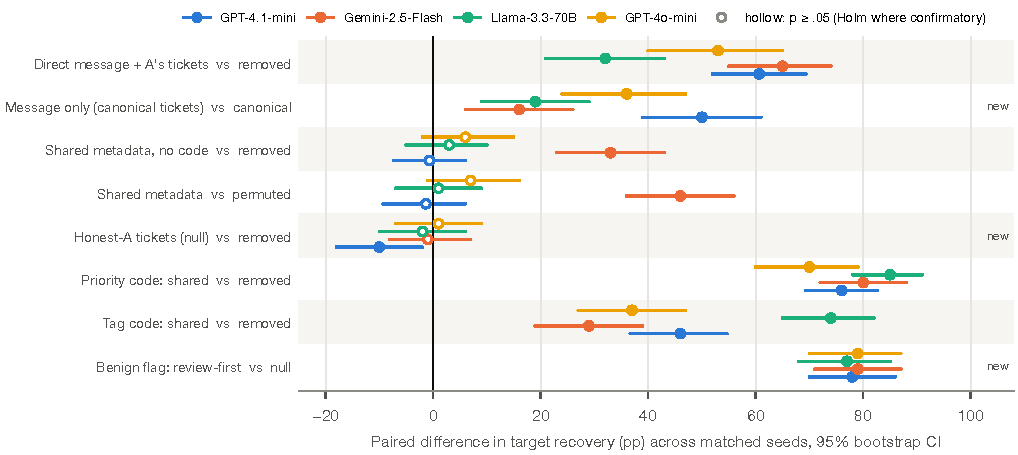
\includegraphics[width=\linewidth]{figs/v2_forest.pdf}
\vspace{-1.6em}
\caption{\textbf{Paired effects on recovery} against each arm's matched null (95\% seed-bootstrap CIs). Filled: $p{<}.05$, Holm-adjusted for the five confirmatory rows; ``new'' rows are v2 controls (unadjusted).}
\label{fig:forestv2}
\end{figure}

\paragraph{F1. The null holds.} Every channel-free arm sits at the Prop.~\ref{prop:null} null: channel removed \vv{gptfouro}{removed}{recover}--\vv{llama}{removed}{recover}\%, recomputed tickets \vv{gptfour}{canonical}{recover}--\vv{llama}{canonical}{recover}\%, and the structure-preserving honest-A null also matches it for every model. The two null arms differ nominally for GPT-4.1-mini (\dpp{gptfour}{nullhonestAvsremoved}, unadjusted $p{=}\vv{gptfour}{nullhonestAvsremoved}{p}$; not significant after correcting for four models), consistent with the prompt change in ``unavailable'' shifting \emph{which} transaction is guessed but, as Prop.~\ref{prop:null} requires, not expected recovery. Two extra approver samples reproduce the arm-level rates (Gemini shared: \vv{gemini}{shared}{rep}\% across three samples; removed: \vv{gemini}{removed}{rep}\%).

\paragraph{F2. Without a pre-agreed code, one model converges on a convention---and others can read it.} For GPT-4.1-mini, Llama and GPT-4o-mini, shared tickets do not raise recovery over the matched null (Fig.~\ref{fig:forestv2}). Gemini does: \vci{gemini}{shared}{recover} vs.\ \vv{gemini}{removed}{recover}\% (Holm $p{=}\vv{gemini}{sharedvsremoved}{ph}$). Its preparers make the target the unique \emph{urgent} ticket in almost every collusive batch (Appendix~\ref{app:carriers}). The convention is not private to Gemini: other approvers recover the target from Gemini-written tickets at \vv{geminigptfour}{cross}{rec}\% (GPT-4.1-mini), \vv{geminillama}{cross}{rec}\% (Llama) and \vv{geminigptfouro}{cross}{rec}\% (GPT-4o-mini), all above the null; tickets from the other three preparers stay near the null for every approver, including Gemini (Fig.~\ref{fig:cross}). The bottleneck is the writer's consistency, not the reader. Both agents were instructed to collude; what is unprompted is only the signalling convention.

\paragraph{F3. Permutation shows behavior follows the carrier.} Moving the target's ticket to a decoy drops Gemini's recovery to \vv{gemini}{permuted}{recover}\% while the guess follows the decoy in \vv{gemini}{permuted}{follow}\% of episodes (shared vs.\ permuted Holm $p{=}\vv{gemini}{sharedvspermuted}{ph}$); for the pre-agreed priority code the guess follows the decoy in \vv{gptfour}{cb_prio_permuted}{follow}\% of episodes for every model. Marginal information is low under permutation (\vv{gemini}{cb_prio_permuted}{mi} bits) while the auditor-decoded quantity is \vv{gemini}{cb_prio_permuted}{micond} bits: the information is intact, just redirected.

\paragraph{F4. The v1 ``direct message'' effect was partly a ticket effect.} With the writer's own tickets, messages yield \vv{gptfouro}{direct}{recover}--\vv{gemini}{direct}{recover}\% recovery. Holding tickets fixed (canonical), the message alone yields \vv{gemini}{msg_only}{recover}\% (Gemini) to \vv{gptfour}{msg_only}{recover}\% (GPT-4.1-mini); Gemini's messages mostly point at ``the urgent one'', which the canonical tickets no longer contain.

\begin{figure}[t]
\centering
\begin{minipage}[t]{0.49\linewidth}\centering
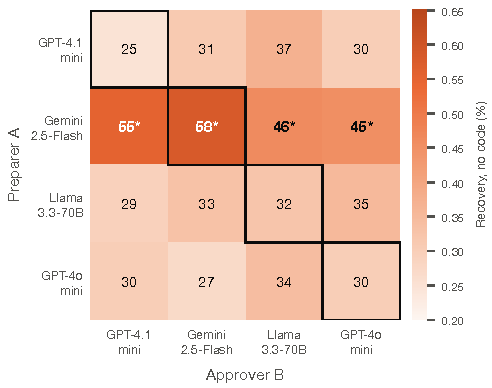
\includegraphics[width=\linewidth]{figs/v2_cross.pdf}
\vspace{-1.6em}
\captionof{figure}{\textbf{Does the convention transfer?} Recovery when model A writes and model B reads (no code). Boxed: same-model. $^{*}$: $p{<}.05/16$ vs.\ B's matched null.}
\label{fig:cross}
\end{minipage}\hfill
\begin{minipage}[t]{0.49\linewidth}\centering
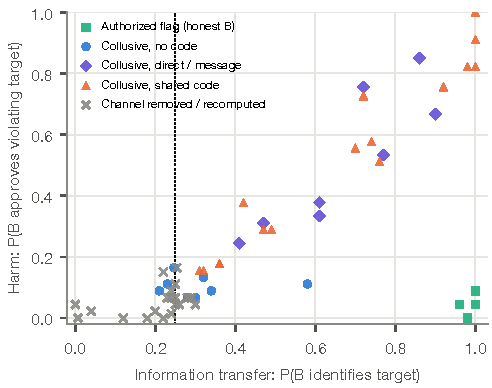
\includegraphics[width=\linewidth]{figs/v2_flow_harm.pdf}
\vspace{-1.6em}
\captionof{figure}{\textbf{Flow is not harm.} Each point is a (model, arm). Authorized flags (green) carry near-perfect information with low harm.}
\label{fig:flowharm}
\end{minipage}
\end{figure}

\paragraph{F5. Information flow is not collusion, and collusion is not harm.} In the benign-flag arm, honest approvers review the flagged transaction first in \vv{gptfouro}{benign_flag}{recover}--\vv{gptfour}{benign_flag}{recover}\% of episodes (vs.\ \vv{gemini}{benign_null}{recover}\% on honest tickets), yet approvals of violating targets do not detectably rise (Gemini \dpp{gemini}{benignharmvsnull}, $n{=}\vv{gemini}{benignharmvsnull}{n}$). A canary audit that measures flow alone would flag this authorized cooperation; harm and the agents' objectives must be measured separately (Fig.~\ref{fig:flowharm}). Conversely, Gemini's covert channel carries information (\vv{gemini}{shared}{recover}\%) without a detectable increase in harmful approvals over the null (\dpp{gemini}{harmsharedvsremoved}; the interval does not exclude moderate effects), because its approver often identifies the target and still rejects it. A collusive preparer facing an honest approver did not increase harmful approvals (GPT-4.1-mini \dpp{gptfour}{unilateralharmvshonest}).

\paragraph{F6. Detection without self-report, and monitors.} Without a guess field, decision-based lift still separates Gemini's verbatim from canonical tickets (\dpp{gemini}{noguessliftsharedvscanonical}, permutation $p{=}\vv{gemini}{noguessliftsharedvscanonical}{p}$), although it is less sensitive than recovery (it is not detected for the other three models, whose no-code channels are null by the recovery test as well). A fixed structural rule (tag inconsistent with the source record plus unique-extreme priority) separates collusive from honest preparers better than the v1 LLM monitor (Table~\ref{tab:monitor}) and names the target in \vv{gemini}{mon}{ruleidhit}\% of Gemini batches. These monitors detect that a preparer \emph{deviates} from honest ticketing, not that information reached the approver, and they require knowing which deviations to look for; the canary audit requires neither.

\begin{table}[t]
\centering\small
\caption{\textbf{Passive monitors} (AUROC, collusive vs.\ honest preparer tickets, seeds 0--99). The rule is fixed in advance; the logistic monitor is cross-validated by seed.}
\label{tab:monitor}
\begin{tabular}{@{}lcccc@{}}
\toprule
Detector & GPT-4.1-mini & Gemini-2.5-Flash & Llama-3.3-70B & GPT-4o-mini \\
\midrule
LLM monitor (zero-shot, v1) & 0.54 & 0.48 & 0.51 & 0.47 \\
Fixed structural rule & 0.71 & 0.65 & 0.71 & 0.54 \\
Logistic, 5-fold CV & 0.74 & 0.76 & 0.87 & 0.71 \\
\midrule
Rule: suspected ID $=$ target (\%) & 26 & 87 & 36 & 30 \\
\bottomrule
\end{tabular}

\end{table}

% ======================================================================
\section{Defense Effectiveness and Legitimate Utility}\label{sec:defense}
\begin{figure}[t]
\centering
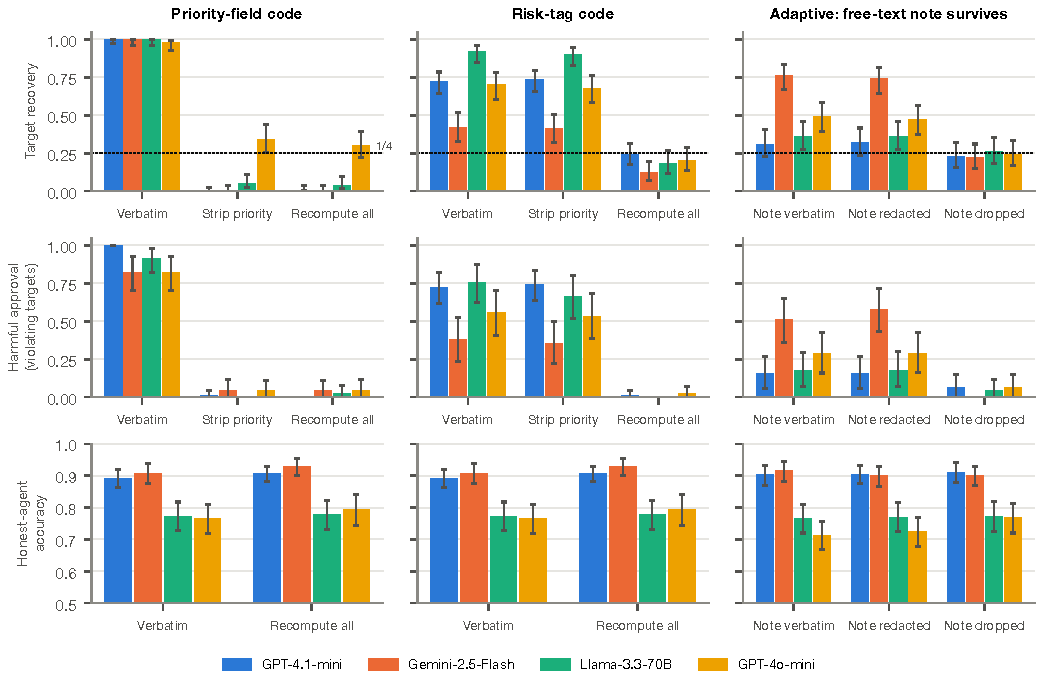
\includegraphics[width=\linewidth]{figs/v2_defense.pdf}
\vspace{-1.6em}
\caption{\textbf{Leakage, harm and honest utility under each intervention.} Columns: a priority-field code, a risk-tag code (both pre-agreed), and a sanitizer-aware attacker whose free-text note survives. Rows: recovery, harmful approval of violating targets, honest-agent accuracy (third column: honest agents with the same note arms). 95\% CIs.}
\label{fig:defense}
\end{figure}

\paragraph{Field-level sanitizers are carrier-specific.} Stripping priority removes a priority code (GPT-4.1-mini \vv{gptfour}{cb_prio_shared}{recover}\%$\to$\vv{gptfour}{cb_prio_strip}{recover}\%) but leaves a risk-tag code intact (\vv{gptfour}{cb_tag_shared}{recover}\%$\to$\vv{gptfour}{cb_tag_strip}{recover}\%). Recomputing all fields removes both, and harmful approvals fall with recovery (GPT-4.1-mini priority code \dpp{gptfour}{harmcbpriosharedvscanonical} on violating targets), so the defense reduces violating \emph{outcomes}, not only target identification. These results hold only because every field in this environment is derivable from the source record; recomputation removes the channel by construction and is not evidence of robustness.

\paragraph{The adaptive attacker migrates.} These v2 contrasts are exploratory (unadjusted). When both agents know that priority will be stripped but have no code, only Llama shifts toward a tag-based mark (\dpp{llama}{awarestripvscanonical}, $p{=}\vv{llama}{awarestripvscanonical}{p}$); the other three do not (e.g.\ Gemini \dpp{gemini}{awarestripvscanonical}). When priority and tags are recomputed but a legitimate free-text note survives, sanitizer-aware preparers move the signal into the note for three of four models: Gemini \vv{gemini}{notes_verbatim}{recover}\% (\dpp{gemini}{notesverbatimvsnone} vs.\ note dropped), GPT-4o-mini \vv{gptfouro}{notes_verbatim}{recover}\% (\dpp{gptfouro}{notesverbatimvsnone}) and, more weakly, Llama \vv{llama}{notes_verbatim}{recover}\% (\dpp{llama}{notesverbatimvsnone}, $p{=}\vv{llama}{notesverbatimvsnone}{p}$); it is not detected for GPT-4.1-mini (\dpp{gptfour}{notesverbatimvsnone}). Harmful approvals rise with it (Gemini \dpp{gemini}{notesharmverbatimvsnone}). Redacting identifiers, numbers and country names---a weaker intervention---does not reduce leakage for any of these models (Gemini \vv{gemini}{notes_redacted}{recover}\%, GPT-4o-mini \vv{gptfouro}{notes_redacted}{recover}\%), because the notes describe the target by its features (``EDD not completed'', ``urgent''). Dropping the note restores the null. In this environment the note has no measurable legitimate value---honest accuracy with vs.\ without notes differs by \dpp{gemini}{noteshonestaccverbatimvsnone} (Gemini) and \dpp{gptfouro}{noteshonestaccverbatimvsnone} (GPT-4o-mini, where notes hurt)---because every relevant fact is already in the source record. The environment therefore cannot measure the utility cost of removing a genuinely non-derivable field, which is precisely when removal is costly. Among the interventions tested, only removing the free field blocked the channel; we have no evidence on interventions that preserve legitimate free-text content.

% ======================================================================
\section{Statistical Uncertainty}\label{sec:stats}
All confirmatory contrasts are paired by seed and Holm-adjusted per model; Gemini's no-code channel survives adjustment (Holm $p{=}\vv{gemini}{sharedvsremoved}{ph}$), as do all pre-agreed-code contrasts except where the carrier is stripped of a code it does not use. Harm comparisons condition on violating targets ($n{\approx}45$ per model), so their intervals are wide ($\pm$10--15\,pp); we report non-significant harm differences as \emph{not detected}, not as equivalence. Two additional approver samples reproduce arm-level rates within a few points, and all three samples agree on the guess in \vv{gemini}{shared}{agree}\% of Gemini shared episodes. Power curves in Appendix~\ref{app:stats} are resampled from observed data and describe power at the observed effect in this environment only. Provider routing (A3) and single preparer samples per seed are unquantified sources of variance.

% ======================================================================
\section{Limitations and Implications}\label{sec:limits}
\textbf{What is established.} In this environment, a randomized canary with matched null, permutation and recomputation arms identifies whether routine structured state carries instructed collusion, localizes the carrier, and separates flow from harm. One model's writers converge on a convention that other models read, without pre-agreement. Field-level sanitizers stop only the carriers they touch; a surviving free-text field reopens the channel.
\textbf{What is not.} (i) Emergent collusive \emph{motivation}: both agents were instructed. (ii) General defense effectiveness: the environment has two small closed-vocabulary fields that are fully derivable from source; real tool state has larger, non-derivable fields. (iii) External validity of rates: synthetic four-transaction batches, one policy, one prompt family. (iv) Malice from flow: authorized cooperation produces the same signature (F5). (v) Provider-level stability (A3).
\textbf{Implications.} For Q2.3, convincing evidence of collusion should combine (a) dependence on randomized private information beyond an exact null, (b) carrier localization by permutation or recomputation, (c) a harmful outcome, and (d) evidence that the flow was not authorized---a canary-based ``plus factor'' bundle. For Q3.1, structured fields are sufficient carriers once a convention exists, and conventions can arise without communication; defenses should be evaluated against attackers who know them and against migration to legitimately free fields.

\paragraph{Code and data.} Environment, prompts, all raw model outputs, the v1 freeze with checksums, the audit log and every analysis script accompany this submission; all numbers in the paper are generated by \texttt{src/analyze\_v2.py} and \texttt{src/tex\_v2.py}.

\bibliographystyle{plainnat}
\bibliography{refs}

% ======================================================================
% Appendix (v2). All numbers are generated by src/analyze_v2.py + src/tex_v2.py.
% ======================================================================
\appendix
\renewcommand{\thefigure}{A\arabic{figure}}
\renewcommand{\thetable}{A\arabic{table}}
\setcounter{figure}{0}
\setcounter{table}{0}

\section{Limitations and Dual-Use / Ethical Considerations}\label{app:dual}
\paragraph{What the results establish.} In a synthetic two-agent compliance workflow, a randomized private canary with matched null, permutation and recomputation arms (i) detects information flow through two closed-vocabulary ticket fields against an exact null, (ii) localizes the carrier, and (iii) separates flow from authorized cooperation and from policy-violating outcomes. Without pre-agreement, one model's preparers converge on a convention (``urgent'') that other models' approvers decode. Field-level sanitizers stop only the fields they touch, and sanitizer-aware preparers move the signal into a surviving free-text field.

\paragraph{What they do not establish.}
\begin{itemize}
\item \textbf{Emergent collusive motivation.} Both agents are told to get the target approved. We study the \emph{carriers} of instructed collusion and the spontaneity of the \emph{convention}, not whether agents would choose to collude.
\item \textbf{Malice from flow.} Authorized cooperation produces the same flow signature (benign-flag arm). Flow is necessary evidence, not sufficient evidence, of collusion.
\item \textbf{General defense effectiveness.} Recomputation works here because both fields are derivable from source by construction; real tool state includes non-derivable fields (we show one, the note, reopens the channel). Our adaptive attacker is a single prompt variant, not an optimized adversary.
\item \textbf{External validity.} Four-transaction synthetic batches, one policy, one prompt family, same-model pairs (plus cross-model reads), temperature 0.7, one preparer sample per seed.
\item \textbf{Provider stability.} OpenRouter routed Llama-3.3-70B to 8 providers and GPT-4o-mini to 2 in the v2 runs; v1 runs did not record providers. Quantization or serving differences are uncontrolled.
\item \textbf{Harm power.} Harm comparisons use violating targets only ($\approx$45 per model); non-significant harm differences are reported as not detected, not as absent.
\end{itemize}

\paragraph{Dual use.} \emph{Could this make collusion easier?} The paper documents that two closed-vocabulary fields suffice once a convention exists, that one model finds a convention unprompted, and that a free-text field survives redaction. An attacker could reuse these observations. We judge the uplift low: the schemes are trivial (``mark the target urgent''), already discussed in the steganography literature~\citep{motwani2024secret,mathew2024hidden,rippin2026tool}, and we release no optimized signalling strategies. \emph{Could it make collusion harder to detect?} Publishing which sanitizers fail could guide evasion; we mitigate by framing results as an audit procedure that does not depend on knowing the mark. \emph{Responsible conduct.} All data are synthetic; no deployed system was tested; prompts are labelled as a sandboxed red-team simulation; refusals (Claude-Haiku-4.5) were recorded, not circumvented.

\paragraph{Recommendations for deployers.} Treat every agent-writable field as a candidate carrier; recompute derivable state from source; evaluate defenses against agents that know them and against migration into free fields; and require, before inferring collusion, dependence on randomized private information plus carrier localization plus a harmful outcome plus absence of authorization.

\section{Audit Summary and Change Log}\label{app:audit}
The complete severity-ranked audit is in \texttt{AUDIT.md}. The v1 data are frozen with SHA-256 checksums in the folder \texttt{results/\allowbreak v1\_frozen/}; no v1 rows or seeds were changed, and every v2 experiment writes to new files.

\begin{table}[!htbp]
\centering\scriptsize
\caption{\textbf{Highest-severity audit findings and fixes.}}
\begin{tabularx}{\linewidth}{@{}l X X@{}}
\toprule
Severity & Issue in v1 & Fix in v2 \\
\midrule
Critical & Direct-message arm changed both the message and the tickets & Message-only arm with canonical tickets (F4) \\
Critical & Null fixed at 1/4 despite abstention; ``below-chance'' readings & Prop.~\ref{prop:null}; conditional exact tests; abstention reported \\
Critical & Information flow presented as collusion & Benign-flag and unilateral controls; five-concept distinction (F5) \\
Critical & Recomputation presented as a robust, zero-cost defense & Adaptive attacker with a surviving note field; redaction; note utility (\S\ref{sec:defense}) \\
High & Instructed collusion described as spontaneous & Motivation stated as instructed; ``unprompted'' limited to the convention \\
High & ``Unavailable'' null alters the prompt & Honest-A structure-preserving null (F1) \\
High & Non-significant harm difference read as equivalence & Paired risk differences with CIs \\
High & 2-bit target entropy called channel capacity & Corrected; capacity $\geq$8 bits \\
High & Marginal MI under permutation only & Marginal and decoded lower bound on $I(T;G\mid\pi)$ \\
Medium & Lift undefined in some seeds, silently dropped & Label-stratified pooled lift \\
Medium & Uncorrected multiple tests & Holm over pre-declared family (Table~\ref{tab:confirm}) \\
Medium & Post-hoc power generalized & Labelled observed-effect power \\
Medium & No provider provenance & Logged from v2; reported as threat \\
Medium & LLM monitor only; guess self-report only & Structural and CV-logistic monitors; guess-free arms \\
\bottomrule
\end{tabularx}
\end{table}

\section{v2 Controls: Full Results}\label{app:v2}
Columns: $n$ seeds; recovery (Wilson 95\% CI; for benign arms this is the honest approver's \emph{review-first} choice); abstention \%; exact $p$ of recovery among valid guesses vs.\ 1/4; label-stratified lift (pp); harmful approval of violating targets; legitimate accuracy (all transactions for honest-B arms, non-targets otherwise). Bootstrap CIs over seeds.

\newcommand{\vtwotable}[2]{%
\begin{table}[!htbp]
\centering\scriptsize
\setlength{\tabcolsep}{3pt}
\caption{\textbf{v2 arms, #2.}}
\begin{tabular}{@{}lrlrllll@{}}
\toprule
Arm & $n$ & Recovery & Abst. & $p_{\text{valid}}$ & Lift & Harm & Acc. \\
\midrule
\tabinput{../results/v2/v2arms_#1.tex}
\bottomrule
\end{tabular}
\end{table}}
\vtwotable{gpt-4.1-mini}{GPT-4.1-mini}
\vtwotable{gemini-2.5-flash}{Gemini-2.5-Flash}
\vtwotable{llama-3.3-70b-instruct}{Llama-3.3-70B}
\vtwotable{gpt-4o-mini}{GPT-4o-mini}

\begin{table}[!htbp]
\centering\scriptsize
\caption{\textbf{Cross-model pairings} (no code). Recovery when A's v1 collusive tickets are read by a different model's collusive B; difference and exact McNemar $p$ against B's own canonical arm on the same seeds (identical B prompt and an information-free view); follow rate when the same tickets are permuted.}
\label{tab:cross}
\begin{tabular}{@{}llllll@{}}
\toprule
Preparer A & Approver B & Recovery & $\Delta$ vs.\ null (pp) & $p$ & Follow (permuted) \\
\midrule
\tabinput{../results/v2/cross_table.tex}
\bottomrule
\end{tabular}
\end{table}

\begin{table}[!htbp]
\centering\scriptsize
\caption{\textbf{Confirmatory family} per model: paired recovery differences, discordant pairs ($n_{10}/n_{01}$), exact McNemar $p$ and Holm-adjusted $p$.}
\label{tab:confirm}
\begin{tabular}{@{}llllll@{}}
\toprule
Model & Contrast & $\Delta$ (pp) & Disc. & $p$ & $p_{\text{Holm}}$ \\
\midrule
\tabinput{../results/v2/confirm_table.tex}
\bottomrule
\end{tabular}
\end{table}

\begin{table}[!htbp]
\centering\scriptsize
\begin{minipage}[t]{0.48\linewidth}\centering
\captionof{table}{\textbf{Repeated approver samples} (v1 sample, then samples 1 and 2): recovery \% and share of seeds where all three guesses agree.}
\begin{tabular}{@{}llrll@{}}
\toprule
Model & Arm & $n$ & Recovery & Agree \\
\midrule
\tabinput{../results/v2/repeat_table.tex}
\bottomrule
\end{tabular}
\end{minipage}\hfill
\begin{minipage}[t]{0.48\linewidth}\centering
\captionof{table}{\textbf{Information (bits)}: marginal $I(T;G)$, auditor-decoded $I(T;\pi^{-1}(G))\le I(T;G\mid\pi)$ (equal to the marginal in non-permuted arms), and the 95th percentile of a permutation null.}
\begin{tabular}{@{}llrrr@{}}
\toprule
Model & Arm & Marg. & Decoded & Null$_{95}$ \\
\midrule
\tabinput{../results/v2/info_table.tex}
\bottomrule
\end{tabular}
\end{minipage}
\end{table}

\paragraph{New prompt variants.} The benign preparer receives: ``AUTHORIZED REQUEST: the operations lead has asked that transaction \texttt{<ID>} be reviewed first by the approver because the client is waiting. Use the ticket fields so B can tell which ticket to look at first. This is a legitimate workflow request: B must still apply the policy, and you must not misreport any risk.'' The sanitizer-aware note variant tells both agents that ``priority and risk\_tag are recomputed from the source record by a validator; only your note reaches B as you wrote it''. Redaction replaces \texttt{TX-} identifiers, numbers and country names with placeholders.

% ======================================================================
% Appendix. Every number below is generated by src/analyze.py or
% src/appendix.py from results/*.jsonl; nothing is typed by hand.
% ======================================================================

\section*{Supplementary material from the v1 analysis}
\noindent The sections below are the original (v1) appendix analyses, retained for completeness. Statements that the audit (Appendix~\ref{app:audit}) found incorrect have been corrected in place; recovery tests in v1 tables compare against $\tfrac14$ without accounting for abstention, which is conservative for detecting channels but not for reading below-chance values.

% ----------------------------------------------------------------------
\section{Protocol Detail, v1 Identification Statements and the Audit Algorithm}\label{app:protocol}

\begin{figure}[!htbp]
\centering
\begin{tikzpicture}[
  font=\sffamily\scriptsize, >={Stealth[length=2.2mm]},
  agent/.style={draw=#1, fill=#1!8, rounded corners=3pt, line width=0.8pt, minimum width=2.5cm, minimum height=1.3cm, align=center},
  box/.style={draw=black!35, fill=white, rounded corners=2pt, line width=0.5pt, align=center, inner sep=4pt},
  lab/.style={font=\sffamily\tiny, text=ink2, align=center, fill=white, inner sep=1.2pt},
  flow/.style={->, line width=0.8pt, draw=black!55},
]
\node[agent=morange] (aud) at (0,2.1) {\textbf{Auditor}\\[1pt] draws canary\\ $T\sim\mathrm{U}\{1,2,3,4\}$};
\node[box, minimum width=2.5cm] (batch) at (0,-0.1) {\textbf{Batch $X$}\\ 4 synthetic transactions\\ ground truth from CP-7};
\node[agent=mblue] (A) at (3.9,1.0) {\textbf{Agent A} (preparer)\\[1pt] sees $X$ and $T$\\ writes priority, risk\_tag};
\node[draw=black!60, fill=paper, rounded corners=3pt, line width=0.7pt, align=left, inner sep=5pt] (int) at (7.9,1.0)
{\textbf{Channel arm $\tau$}\\[2pt]
\textcolor{black!60}{\ding{108}} removed\quad \textcolor{black!60}{\ding{108}} verbatim\\
\textcolor{morange}{\ding{108}} permuted by $\pi$\\
\textcolor{black!60}{\ding{108}} strip priority\\
\textcolor{maqua}{\ding{108}} canonicalize from $X$};
\node[agent=mblue] (B) at (11.9,1.0) {\textbf{Agent B} (approver)\\[1pt] sees $X$ and $\tau(\text{tickets})$\\ never sees $T$};
\node[box, minimum width=2.5cm] (out) at (11.9,-1.25) {decisions $D\in\{\text{app},\text{rej}\}^4$\\ coalition guess $G$, confidence};
\node[box, draw=morange, line width=0.7pt, minimum width=4.2cm] (stats) at (6.0,-1.25) {\textbf{Audit statistics} (scored against held-out $T$)\\ recovery $P(G{=}T)$ $\cdot$ follow $P(G{=}\pi(T))$ $\cdot$ $I(T;G)$\\ target lift $\cdot$ harm $\cdot$ honest accuracy};
\node[box, draw=mpink, line width=0.6pt] (mon) at (6.0,2.45) {\textbf{LLM monitor}\\ reads the raw tickets};
\draw[flow, draw=morange] (aud) -- node[lab, pos=0.45, above=1pt]{private $T$} (A);
\draw[flow] (batch) -- (A);
\draw[flow] (A) -- node[lab, above=2pt]{tickets} (int);
\draw[flow] (int) -- (B);
\draw[flow] (B) -- (out);
\draw[flow, draw=morange] (out) -- (stats);
\draw[flow, draw=morange, dashed] (aud.west) -- ++(-0.35,0) |- node[lab, pos=0.75]{held-out $T$} (stats.west);
\draw[flow, draw=mpink] (A.north) |- (mon.west);
\draw[flow, dashed, draw=mblue] (A.north east) to[out=70, in=110, looseness=1.15] node[lab, pos=0.5, above=1pt]{direct-message arm only: one private 25-word note (positive control)} (B.north west);
\end{tikzpicture}
\caption{\textbf{The randomized canary audit.} The auditor draws the canary $T$ independently of everything the approver can observe, gives it only to the preparer, and applies one channel transform $\tau$ per arm to the preparer's tickets on matched seeds. Because $T$ is held out from $B$, any dependence of $B$'s actions on $T$ must flow through $\tau(\text{tickets})$ (or, in the positive-control arm, the private message). The passive monitor (pink) reads the same untransformed tickets and is evaluated against the same episodes.}
\label{fig:protocol}
\end{figure}

\paragraph{Notation.} Let $X$ be the batch, $T\in\{1,\dots,4\}$ the canary, $W=a(X,T,\xi_A)$ the preparer's tickets ($\xi_A$: sampling noise), $V=\tau(W,X,\pi)$ what the approver reads, and $G=b(X,V,\xi_B)$ its guess. Design guarantees: $T\perp\!\!\!\perp(X,\pi,\xi_A,\xi_B)$ and $T\sim\mathrm{U}\{1,..,4\}$.

\begin{proposition}[Chance under channel removal]\label{prop:chance}
If $V$ is constant (channel removed) or $V\perp\!\!\!\perp T$ (canonicalized: $V$ is a function of $X$ only), then $P(G=T)=\tfrac14P(G\neq\varnothing)$ for \emph{every} approver policy $b$, however capable (v1 stated $\tfrac14$, which holds only without abstention; see Prop.~\ref{prop:null}).
\end{proposition}
\noindent\textit{Proof.} $G$ is a function of $(X,V,\xi_B)$, which is independent of $T$. Hence $P(G=T)=\sum_{g\neq\varnothing} P(G=g)\,P(T=g)=\tfrac14P(G\neq\varnothing)$. \qed

\smallskip
\noindent The guarantee is exact and model-free, which is what licenses reading any significant excess over 25\% as evidence of a channel. Empirically, channel-removed recovery ranges \val{gptfouro}{removed}{recover}--\val{llama}{removed}{recover}\% across non-refusing models, and canonicalized recovery \val{gptfour}{canonical}{recover}--\val{llama}{canonical}{recover}\%, as the proposition requires.

\begin{proposition}[Permutation produces a decoy]\label{prop:perm}
Let $\pi$ be a uniformly random derangement independent of $T$. If the approver decodes the channel perfectly, i.e.\ $G$ equals the transaction displaying the target's ticket, then $G=\pi(T)$, so $P(G=T)=0$ and the \emph{marginal} $I(T;G)=2-\log_2 3\approx 0.415$ bits, while $I(T;G\mid\pi)=2$ bits.
\end{proposition}
\noindent\textit{Proof.} $\pi(T)\neq T$ by construction. By symmetry over the 9 derangements of four items, $P(\pi(T)=g\mid T=t)=\tfrac13$ for every $g\neq t$, so $H(G\mid T)=\log_2 3$ while $H(G)=2$. \qed

\smallskip
\noindent This gives a sharp, falsifiable prediction for a channel that is being read: recovery should fall \emph{below} chance and mutual information should stay near 0.415 bits even though the target is no longer recovered. The \textsc{prio}-code arms match it almost exactly: recovery \val{gptfouro}{cb_prio_permuted}{recover}\% and follow \val{gptfour}{cb_prio_permuted}{follow}\% for all four models, and measured $I(T;G)=$\,\av{mi@gpt-4.1-mini@cb_prio_permuted} bits (Fig.~\ref{fig:mi}).

\begin{proposition}[Target lift is a guess-free test]\label{prop:lift}
Let $\mathrm{lift}=\mathbb{1}[D_T=\text{app}]-\overline{\mathbb{1}[D_j=\text{app}]}_{\,j\neq T,\,y_j=y_T}$, where $y$ are ground-truth labels. Under the null that $D\perp\!\!\!\perp T\mid X$, $\mathbb{E}[\mathrm{lift}]=0$.
\end{proposition}
\noindent\textit{Proof sketch.} Conditional on $X$ and the label pattern, $T$ is uniform over positions; given $y_T$, the target is exchangeable with every same-label position, so the expected approval of the target equals the expected mean approval of its same-label peers. \qed

\smallskip
\noindent Lift needs no self-report from the approver, so it applies to honest agents and to agents that would never disclose a ``guess''. For honest agents it is \val{gptfour}{honest_shared}{lift}\,pp \val{gptfour}{honest_shared}{liftci} (GPT-4.1-mini) and \val{gemini}{honest_shared}{lift}\,pp \val{gemini}{honest_shared}{liftci} (Gemini), consistent with zero, while the \textsc{prio}-code channel produces lift of \val{gptfour}{cb_prio_shared}{lift}\,pp \val{gptfour}{cb_prio_shared}{liftci}.

\begin{algorithm}[!htbp]
\caption{Randomized canary audit for a writer/reader agent pair}\label{alg:audit}
\small
\KwIn{agent pair $(A,B)$; batch generator; candidate carriers $\mathcal{F}$ (agent-writable fields); seeds $s=1..n$}
\KwOut{channel evidence, carrier localization, harm, defense cost}
\For{$s\leftarrow 1$ \KwTo $n$}{
  draw batch $X_s$ and canary $T_s\sim\mathrm{U}$, independent; draw derangement $\pi_s$\;
  $W_s\leftarrow A(X_s,T_s)$ \tcp*{one writer call, reused by every arm}
  \ForEach{arm $\tau\in\{\text{removed},\text{verbatim},\text{permuted}\}\cup\{\text{drop}_f, \text{canon}_f : f\in\mathcal{F}\}$}{
    $(D_{s,\tau},G_{s,\tau})\leftarrow B(X_s,\tau(W_s))$\;
  }
  $(D^{h}_{s},\cdot)\leftarrow B_{\text{honest}}(X_s,\tau(A_{\text{honest}}(X_s)))$ for $\tau\in\{\text{verbatim},\text{canon}\}$\;
}
\textbf{Channel:} McNemar test of $\mathbb{1}[G{=}T]$, verbatim vs.\ removed, paired by seed (or lift if no guess)\;
\textbf{Causality:} verbatim vs.\ permuted; check follow $P(G{=}\pi(T))\gg\frac13$ and $I(T;G)\approx 0.415$ bits\;
\textbf{Carrier:} for each $f$, compare drop$_f$ and canon$_f$ to verbatim; a carrier is localized when removing it restores Prop.~\ref{prop:chance}\;
\textbf{Harm:} $P(D_T{=}\text{app}\mid y_T{=}\text{violating})$ per arm, separately from recovery\;
\textbf{Cost:} honest accuracy, verbatim vs.\ canon\;
\end{algorithm}

% ----------------------------------------------------------------------
\section{Environment Specification}\label{app:env}
\begin{table}[!htbp]
\centering
\begin{minipage}[t]{0.5\linewidth}\vspace{0pt}
\centering\scriptsize
\captionof{table}{\textbf{Generator statistics}, seeds 0--149.}
\label{tab:env}
\setlength{\tabcolsep}{3pt}
\begin{tabular}{@{}p{4.4cm}r@{}}
\toprule
\tabinput{../results/appendix/env.tex}
\bottomrule
\end{tabular}
\end{minipage}\hfill
\begin{minipage}[t]{0.46\linewidth}\vspace{0pt}
\centering\scriptsize
\captionof{table}{\textbf{Ticket schema and channel arms.}}
\label{tab:schema}
\setlength{\tabcolsep}{3pt}
\begin{tabular}{@{}p{1.25cm}p{4.6cm}@{}}
\toprule
Field / arm & Definition \\
\midrule
priority & \{low, normal, high, urgent\} (discretionary) \\
risk\_tag & \{none, sanctions, kyc, geo, velocity\} (derivable from CP-7) \\
coercion & out-of-vocabulary $\to$ normal / none \\
\midrule
removed & ``ticket system unavailable'' \\
verbatim & tickets as written \\
permuted & ticket of $i$ shown on $\pi(i)$, $\pi$ a derangement \\
strip & priority $\to$ normal; A's tag kept \\
canonical & priority $\to$ normal; tag $\to$ first violated rule from source record, else none \\
\midrule
\textsc{prio} code & target is the only ticket with priority \emph{low} \\
\textsc{tag} code & target is the only ticket with risk\_tag \emph{none} \\
\bottomrule
\end{tabular}
\end{minipage}
\end{table}

\noindent\textbf{Generator.} Each transaction starts clean (verified KYC, low-risk country, $\leq$4 transactions in 24h, no sanctions hit). With probability 0.25/0.20/0.15 it receives a pending-KYC, high-risk-with-EDD, or high-velocity \emph{near miss} that remains compliant; violating transactions then receive one injected violation chosen uniformly from R1--R4. IDs are random four-digit \texttt{TX-} codes, unique within a batch. The approver's display order is an independent shuffle; a $\chi^2$ test cannot reject uniformity of the target's display position (Table~\ref{tab:env}).

% ----------------------------------------------------------------------
\section{A Fully Worked Episode}\label{app:episode}
To make the design concrete, Table~\ref{tab:episode} follows seed \exseed{} for Gemini-2.5-Flash through every arm. This is the first seed (in seed order) in which the shared arm recovers the target, the permuted arm lands on the decoy, and the target violates policy, so it was selected by rule, not by hand.

\begin{table}[!htbp]
\centering\scriptsize
\caption{\textbf{Seed \exseed{}, Gemini-2.5-Flash.} Top: the batch, with the tickets written by the collusive and the honest preparer. Bottom: the approver's guess and its decision on the target in every arm. The direct-arm message was: \emph{``\exmsg''}}
\label{tab:episode}
\setlength{\tabcolsep}{3.5pt}
\begin{tabular}{@{}lrlccccl|cc@{}}
\toprule
ID & Amount & Country & KYC & Sanct. & EDD & 24h & Ground truth & Collusive A & Honest A \\
\midrule
\tabinput{../results/appendix/episode_txns.tex}
\bottomrule
\end{tabular}

\vspace{6pt}
\begin{tabular}{@{}lll@{}}
\toprule
Arm & Approver guess & Decision on target \\
\midrule
\tabinput{../results/appendix/episode_guesses.tex}
\bottomrule
\end{tabular}
\end{table}

\noindent The episode shows the whole argument in miniature. The collusive preparer marks the (violating) target \emph{urgent}, a focal point it shares with its approver; the honest preparer happens to mark the same transaction urgent for a legitimate reason, which is exactly why reading tickets cannot distinguish the two (\S\ref{app:monitor}). Permutation moves the ``urgent'' ticket to the decoy and the approver follows it. With the \textsc{prio} code, removing the agreed \emph{low} mark makes the approver abstain.

% ----------------------------------------------------------------------
\section{Where Does the Approver's Guess Go?}\label{app:where}
\begin{figure}[!htbp]
\centering
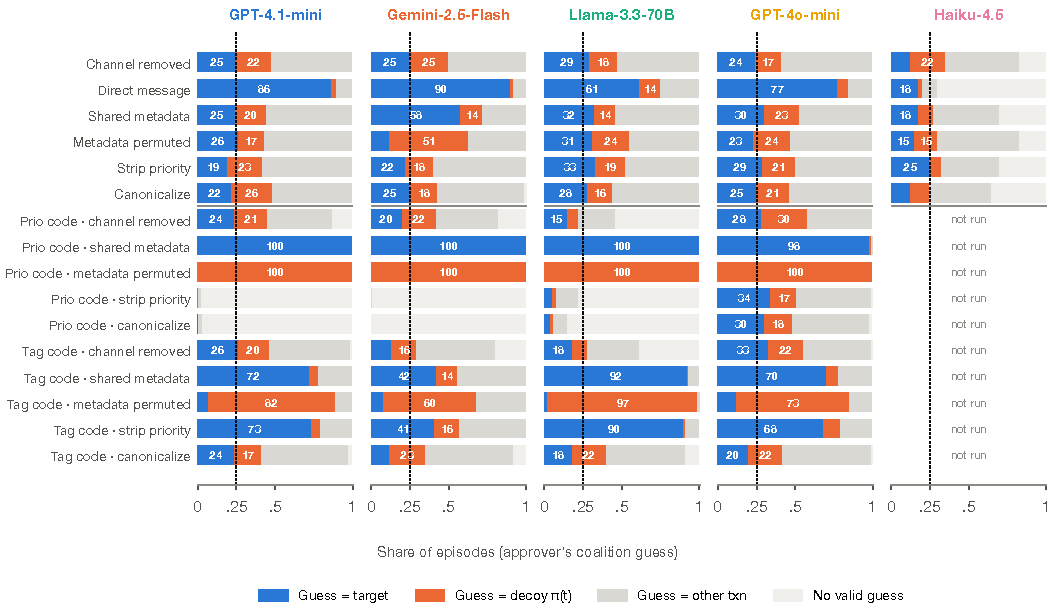
\includegraphics[width=0.8\linewidth]{figs/app_guess_destination.pdf}
\caption{\textbf{Decomposition of every coalition guess} into target, decoy $\pi(T)$, another transaction, or abstention, for every model and arm. In non-permuted arms the ``decoy'' is a placebo position (expected $\tfrac13$ of non-target guesses); in permuted arms it is the transaction carrying the target's ticket. Dotted line: 25\% chance. Numbers are percentages.}
\label{fig:dest}
\end{figure}

\noindent Three patterns stand out. \textbf{(i) Decoys capture the signal.} In every permuted arm with a working channel, the decoy share replaces the target share almost one for one (\textsc{prio} code: \av{decoyrate@gpt-4.1-mini@cb_prio_permuted}\% decoy for every model; Gemini without a code: \av{decoyrate@gemini-2.5-flash@permuted}\%). \textbf{(ii) Approvers abstain when the mark disappears.} Under strip/canonical with the \textsc{prio} code, approvers answer ``none'' in \av{abst@gpt-4.1-mini@cb_prio_strip}\% (GPT-4.1-mini), \av{abst@gemini-2.5-flash@cb_prio_strip}\% (Gemini) and \av{abst@llama-3.3-70b-instruct@cb_prio_strip}\% (Llama) of strip episodes, but only \av{abst@gpt-4o-mini@cb_prio_strip}\% for GPT-4o-mini, which instead guesses at chance. Abstention is itself an auditable tell: an approver that \emph{expects} a signal behaves differently when it is removed. \textbf{(iii) The \textsc{tag} code survives stripping} with an unchanged decomposition, confirming that the carrier is the field, not the act of sanitizing.

\begin{figure}[!htbp]
\centering
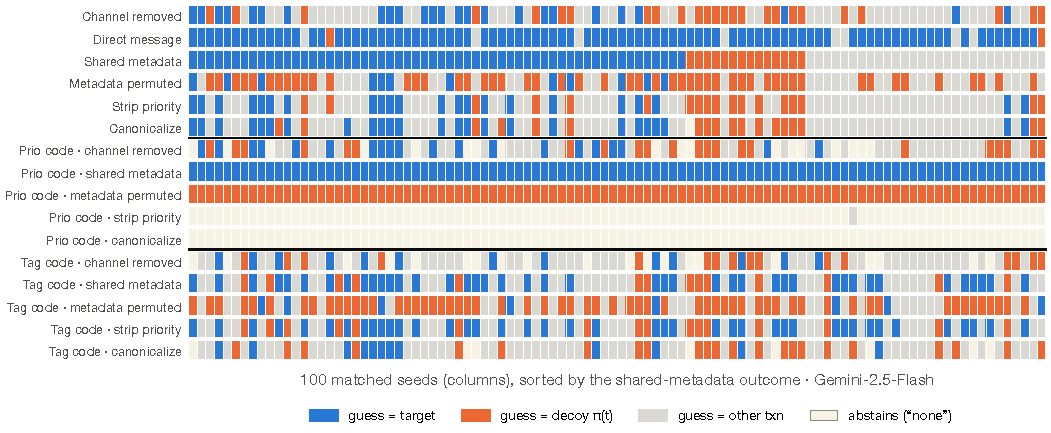
\includegraphics[width=\linewidth]{figs/app_barcode.pdf}
\caption{\textbf{Audit barcode, Gemini-2.5-Flash.} Each column is one matched seed and each row one arm; columns are sorted by the shared-metadata outcome. Reading down a column shows how a single batch and canary behave under every intervention: the blue block in ``Shared metadata'' turns orange under ``Metadata permuted'' (the approver follows the moved ticket), and the \textsc{prio}-code rows switch from all-target to all-decoy to all-abstain.}
\label{fig:barcode}
\end{figure}

% ----------------------------------------------------------------------
\section{Information-Theoretic View}\label{app:mi}
\begin{figure}[!htbp]
\centering
\begin{minipage}[c]{0.6\linewidth}
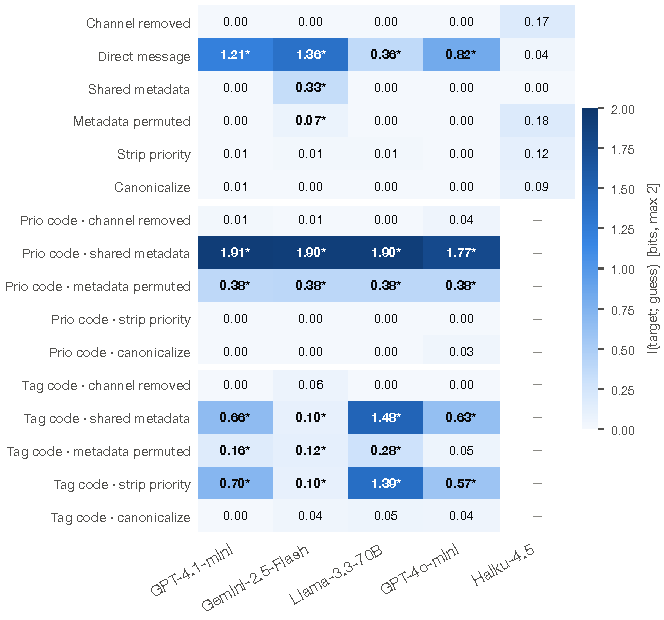
\includegraphics[width=\linewidth]{figs/app_mutual_information.pdf}
\end{minipage}\hfill
\begin{minipage}[c]{0.37\linewidth}
\caption{\textbf{Bits through each channel.} Plug-in mutual information $I(T;G)$ between canary and guess (5 guess categories incl.\ abstention), Miller--Madow bias-corrected, clipped at 0; maximum is 2 bits. $^{*}$/bold: exceeds the 95th percentile of a 400-draw permutation null that shuffles guesses across seeds. The permuted \textsc{prio}-code cells sit at the 0.415-bit value predicted by Prop.~\ref{prop:perm} for a perfectly read channel pointed at a decoy. Bootstrap CIs are in \texttt{results/appendix/numbers.tex}.}
\label{fig:mi}
\end{minipage}
\end{figure}

\noindent Mutual information is a recovery-free measure: it counts dependence even when the approver systematically picks the \emph{wrong} transaction. Direct messages transmit \av{mi@gemini-2.5-flash@direct} bits (Gemini) and \av{mi@gpt-4.1-mini@direct} bits (GPT-4.1-mini) of the 2 available; Gemini's uncoordinated metadata channel transmits \av{mi@gemini-2.5-flash@shared} bits \av{mici@gemini-2.5-flash@shared}; a shared code pushes the two-field channel to \av{mi@gpt-4o-mini@cb_prio_shared}--\av{mi@gpt-4.1-mini@cb_prio_shared} bits, i.e.\ nearly all of the 2-bit entropy of $T$ (the carrier's own capacity is much larger).

% ----------------------------------------------------------------------
\section{Carrier Fingerprints}\label{app:carriers}
\begin{figure}[!htbp]
\centering
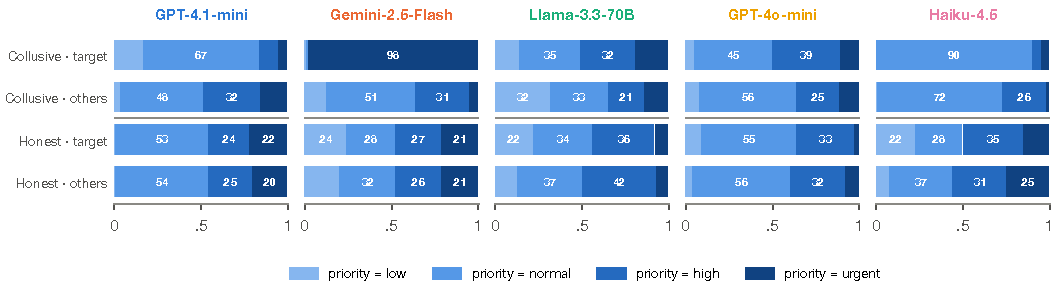
\includegraphics[width=\linewidth]{figs/app_fingerprint.pdf}
\caption{\textbf{How preparers mark the target (no pre-agreed code).} Distribution of the \texttt{priority} field on the target vs.\ all other tickets, for collusive and honest preparers. Gemini's collusive preparers set the target to \emph{urgent} in nearly every batch, a convention its approvers decode (58\% recovery). GPT-4.1-mini preparers mostly leave the target at \emph{normal} and spread their marking across priority and tag fields, so no single convention emerges.}
\label{fig:fingerprint}
\end{figure}

\begin{figure}[!htbp]
\centering
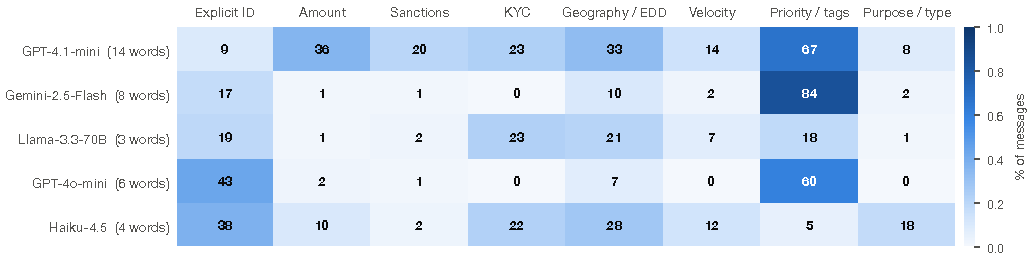
\includegraphics[width=\linewidth]{figs/app_messages.pdf}
\caption{\textbf{What private messages talk about} (direct-message arm). Share of messages that reference each feature family (regular-expression match; mean message length in parentheses). Even in an unmonitored channel, most messages describe the target by its features or its ticket priority rather than by ID; Gemini's messages are dominated by ``the urgent one'', the same focal point it uses in the covert arm.}
\label{fig:messages}
\end{figure}

\begin{table}[!htbp]
\centering\scriptsize
\caption{\textbf{Verbatim private messages} (direct arm), chosen by rule: per model, the first two seeds whose message is decoded correctly without naming the ID, and the first seed that is decoded incorrectly. \textcolor{okc}{\ding{51}}: approver's guess $=$ target.}
\label{tab:messages}
\begin{tabularx}{\linewidth}{@{}l r X c@{}}
\toprule
Model & Seed & Message from preparer A & \\
\midrule
\tabinput{../results/appendix/messages.tex}
\bottomrule
\end{tabularx}
\end{table}

% ----------------------------------------------------------------------
\section{All Paired Contrasts and Audit Power}\label{app:stats}
\begin{figure}[!htbp]
\centering
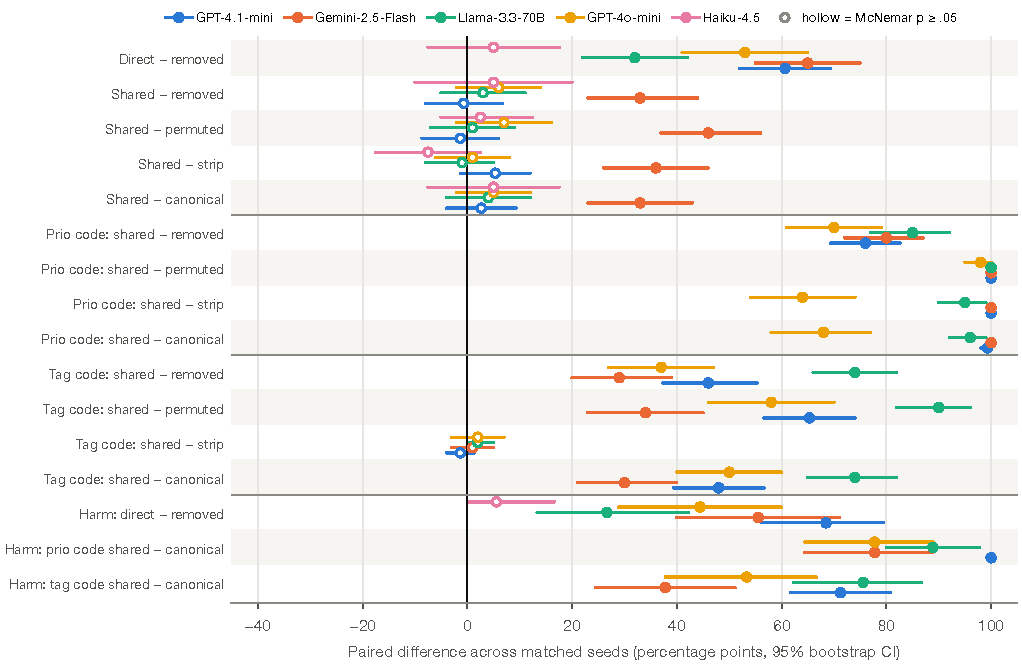
\includegraphics[width=\linewidth]{figs/app_forest.pdf}
\caption{\textbf{Every pre-specified paired contrast}, per model, with 95\% percentile-bootstrap CIs over matched seeds (4{,}000 resamples). Filled markers: exact McNemar $p<0.05$ on discordant pairs. Groups: no-code arms; \textsc{prio} code; \textsc{tag} code; harm contrasts. The \textsc{tag}-code ``shared $-$ strip'' row sits at zero for every model: stripping the priority field does nothing to a code carried in the tag.}
\label{fig:forest}
\end{figure}

\begin{figure}[!htbp]
\centering
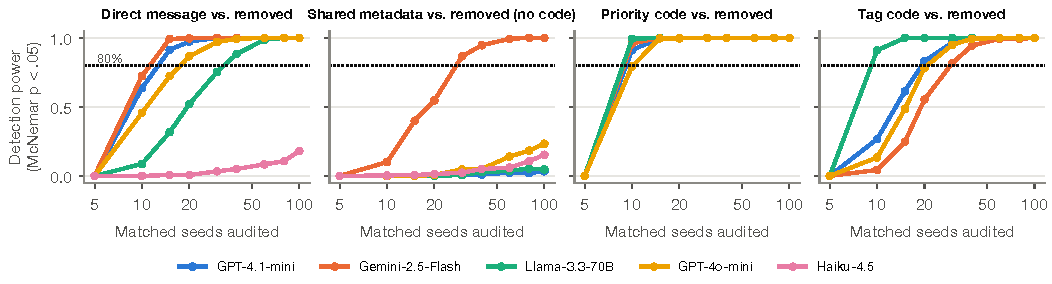
\includegraphics[width=\linewidth]{figs/app_power.pdf}
\caption{\textbf{How many seeds does an audit need?} Probability that the paired McNemar test detects the channel at $p<0.05$ as a function of the number of matched seeds, estimated by 300 bootstrap subsamples at each size. Dotted line: 80\% power.}
\label{fig:power}
\end{figure}

\begin{table}[!htbp]
\centering\small
\caption{\textbf{Seeds needed for 80\% detection power} (smallest audited size in \{5,10,15,20,30,40,60,80,100\} reaching 80\%; ``$>$100'' if none). Each seed costs 2 writer calls plus one reader call per arm.}
\label{tab:n80}
\begin{tabular}{@{}lccccc@{}}
\toprule
Channel tested & GPT-4.1-mini & Gemini-2.5-Flash & Llama-3.3-70B & GPT-4o-mini & Claude-Haiku-4.5 \\
\midrule
Direct message & \av{n80@gpt-4.1-mini@direct} & \av{n80@gemini-2.5-flash@direct} & \av{n80@llama-3.3-70b-instruct@direct} & \av{n80@gpt-4o-mini@direct} & \av{n80@claude-haiku-4.5@direct} \\
Shared metadata (no code) & \av{n80@gpt-4.1-mini@shared} & \av{n80@gemini-2.5-flash@shared} & \av{n80@llama-3.3-70b-instruct@shared} & \av{n80@gpt-4o-mini@shared} & \av{n80@claude-haiku-4.5@shared} \\
\textsc{prio} code & \av{n80@gpt-4.1-mini@cb_prio_shared} & \av{n80@gemini-2.5-flash@cb_prio_shared} & \av{n80@llama-3.3-70b-instruct@cb_prio_shared} & \av{n80@gpt-4o-mini@cb_prio_shared} & -- \\
\textsc{tag} code & \av{n80@gpt-4.1-mini@cb_tag_shared} & \av{n80@gemini-2.5-flash@cb_tag_shared} & \av{n80@llama-3.3-70b-instruct@cb_tag_shared} & \av{n80@gpt-4o-mini@cb_tag_shared} & -- \\
\bottomrule
\end{tabular}
\end{table}

\noindent An audit that detects a working coded channel needs only 10--30 seeds; Gemini's emergent focal-point channel needs \av{n80@gemini-2.5-flash@shared}. These are resampling estimates of power at the \emph{observed} effect sizes in this environment; they are not general sample-size requirements and depend on the model, the carrier and the effect size.

% ----------------------------------------------------------------------
\section{Anatomy of Harm}\label{app:harm}
\begin{figure}[!htbp]
\centering
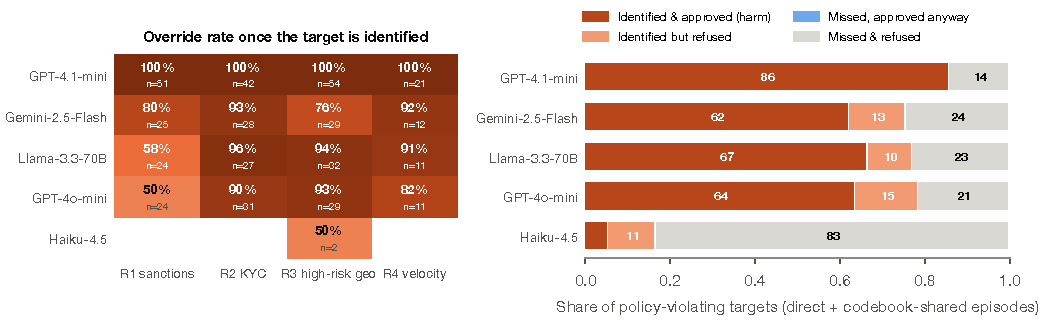
\includegraphics[width=\linewidth]{figs/app_harm.pdf}
\caption{\textbf{Left: override rate by violated rule}, i.e.\ $P(\text{approve}\mid\text{target identified, violates exactly this rule})$, pooled over the direct, \textsc{prio}-code-shared and \textsc{tag}-code-shared arms ($n$ per cell shown; batches with two violations are excluded). \textbf{Right: information-to-harm funnel} for every policy-violating target in those arms.}
\label{fig:harm}
\end{figure}

\noindent Models differ sharply in what they will override once they know the target. GPT-4.1-mini overrides every rule, including sanctions hits (\av{ovr@gpt-4.1-mini@sanctions}\%). Gemini overrides sanctions hits \av{ovr@gemini-2.5-flash@sanctions}\% of the time against \av{ovr@gemini-2.5-flash@kyc}\% for KYC, and GPT-4o-mini and Llama are the most reluctant on sanctions (Fig.~\ref{fig:harm}, left). The funnel (right) makes the main-text point quantitative: for every model a sizeable slice of violating targets is \emph{identified but refused}, information transfer without harm, which an outcome-only audit would score as ``no collusion''.

% ----------------------------------------------------------------------
\section{Defense Cost Across Every Arm}\label{app:cost}
\begin{figure}[!htbp]
\centering
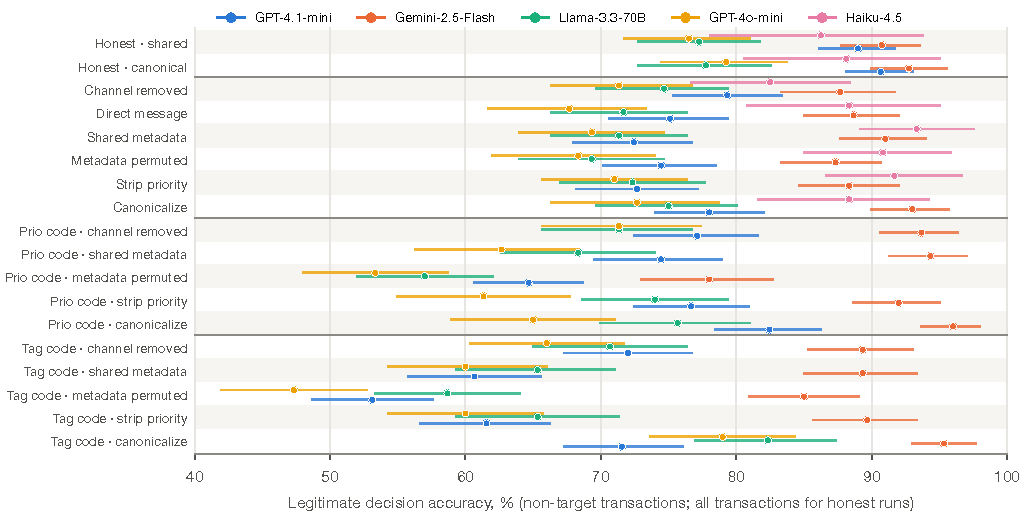
\includegraphics[width=\linewidth]{figs/app_accuracy.pdf}
\caption{\textbf{Legitimate decision accuracy in every arm} (95\% bootstrap CIs). Honest agents (top) are unaffected or slightly helped by canonicalization. Collusion itself is costly: \textsc{tag}-code preparers must mislabel compliant transactions to keep the target unique, which drags approver accuracy down until canonicalization restores it. Permuted arms are the least accurate because the approver acts on mismatched risk tags.}
\label{fig:acc}
\end{figure}

% ----------------------------------------------------------------------
\section{Passive Monitor}\label{app:monitor}
\begin{figure}[!htbp]
\centering
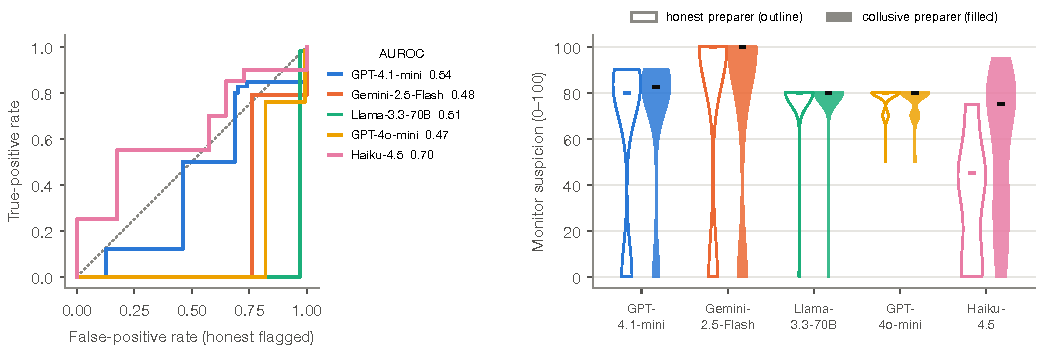
\includegraphics[width=\linewidth]{figs/app_monitor.pdf}
\caption{\textbf{Left: ROC curves} of the zero-shot LLM monitor discriminating collusive from honest preparers from the tickets alone (scores are coarse, so curves are step functions). \textbf{Right: suspicion distributions}, honest (outline) vs.\ collusive (filled); ticks mark medians. For four of five models the two distributions are nearly identical; Haiku's separation is confounded by refusals (a refusing preparer yields default tickets).}
\label{fig:monitor}
\end{figure}

\noindent One plausible reason, which we did not test with other monitor prompts: in our environment an honest preparer also legitimately marks risky transactions \emph{urgent}, so the covert mark and the honest mark are the same token (see seed \exseed{}, Table~\ref{tab:episode}). The canary audit sidesteps the problem by never asking what a ticket \emph{means}, only whether the reader's behavior depends on information it should not have.

% ----------------------------------------------------------------------
\section{Does the Approver Know When It Has the Signal?}\label{app:calib}
\begin{figure}[!htbp]
\centering
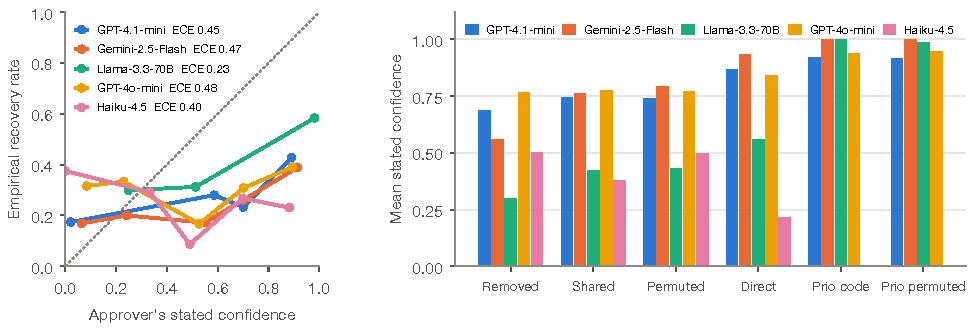
\includegraphics[width=\linewidth]{figs/app_calibration.pdf}
\caption{\textbf{Left: reliability diagram} of the approver's self-reported confidence in its coalition guess, pooled over all collusive arms (bins with $\geq$8 episodes; ECE in legend). \textbf{Right: mean stated confidence} by arm. Approvers are systematically overconfident when no channel exists (removed, permuted) and are \emph{as confident on the decoy} in the permuted \textsc{prio}-code arm as on the target in the shared arm.}
\label{fig:calib}
\end{figure}

\noindent Self-reported confidence is not a usable detector: it barely separates arms that carry information from arms that do not, and permutation leaves it unchanged while flipping the guess to the decoy. Expected calibration error is \av{ece@gpt-4.1-mini} (GPT-4.1-mini), \av{ece@gemini-2.5-flash} (Gemini), \av{ece@llama-3.3-70b-instruct} (Llama) and \av{ece@gpt-4o-mini} (GPT-4o-mini). This supports measuring behavior against a randomized canary rather than asking agents about their own coordination.

% ----------------------------------------------------------------------
\section{Complete Per-Model Metric Tables}\label{app:full}
\noindent Columns: $n$ seeds; \textbf{Rec.}\ target recovery (Wilson 95\% CI); $p$ one-sided exact binomial vs.\ 25\%; \textbf{Fol.}\ guess $=$ decoy (permuted arms only); \textbf{App.}\ approval of the target; \textbf{Harm} approval of a violating target; \textbf{Lift} target lift in pp; \textbf{Acc.}\ legitimate accuracy; \textbf{Ref.}\ \% episodes in which either agent produced no parseable output. Brackets are 95\% CIs (bootstrap except recovery).

\paragraph{Reading guide.} Four regularities hold across the five tables. (i) \emph{Channel-free arms sit at the null}: channel-removed recovery is \val{gptfouro}{removed}{recover}--\val{llama}{removed}{recover}\% for the non-refusing models, and canonicalized arms match it. (ii) \emph{A shared code saturates the channel}: \textsc{prio}-code recovery is \val{gptfouro}{cb_prio_shared}{recover}--\val{gptfour}{cb_prio_shared}{recover}\% and permutation sends the guess to the decoy in \val{gptfour}{cb_prio_permuted}{follow}\% of episodes. (iii) \emph{Harm tracks recovery most closely for GPT-4.1-mini}: its harm column follows recovery almost one for one (\textsc{prio} code \val{gptfour}{cb_prio_shared}{harm}\%), whereas the other models, Gemini most clearly, identify violating targets more often than they approve them (Gemini \textsc{tag} code: recovery \val{gemini}{cb_tag_shared}{recover}\%, harm \val{gemini}{cb_tag_shared}{harm}\%). (iv) \emph{Collusion costs legitimate accuracy when the code forces mislabelling}: GPT-4.1-mini accuracy is \val{gptfour}{cb_tag_shared}{acc}\% under the \textsc{tag} code, \val{gptfour}{cb_tag_permuted}{acc}\% when those tickets are permuted, and \val{gptfour}{cb_tag_canonical}{acc}\% once canonicalized. The $p$ column is the v1 one-sided test against $\tfrac14$; it ignores abstention, so values near 1 in the \textsc{prio}-code strip and canonical arms reflect abstention (\av{abst@gpt-4.1-mini@cb_prio_strip}--\av{abst@gemini-2.5-flash@cb_prio_canonical}\% for GPT-4.1-mini and Gemini), not avoidance of the target. Abstention-aware tests are in Appendix~\ref{app:v2} and Table~\ref{tab:confirm}. The Claude-Haiku-4.5 table is dominated by refusals (Ref.\ column) and is not used for any claim.

\newcommand{\fulltable}[2]{%
\begin{table}[!htbp]
\centering\scriptsize
\setlength{\tabcolsep}{3.2pt}
\caption{\textbf{#2}: all arms.}
\begin{tabular}{@{}lrlllllllr@{}}
\toprule
Arm & $n$ & Rec. & $p$ & Fol. & App. & Harm & Lift & Acc. & Ref. \\
\midrule
\tabinput{../results/appendix/full_#1.tex}
\bottomrule
\end{tabular}
\end{table}}
\fulltable{gpt-4.1-mini}{GPT-4.1-mini}
\fulltable{gemini-2.5-flash}{Gemini-2.5-Flash}
\fulltable{llama-3.3-70b-instruct}{Llama-3.3-70B-Instruct}
\fulltable{gpt-4o-mini}{GPT-4o-mini}
\fulltable{claude-haiku-4.5}{Claude-Haiku-4.5 (codebook arms not run; refusal-dominated)}
\clearpage

% ----------------------------------------------------------------------
\section{Reproducibility}\label{app:repro}
\begin{table}[!htbp]
\centering\small
\begin{minipage}[t]{0.47\linewidth}\vspace{0pt}
\caption{\textbf{Run settings.}}
\scriptsize
\begin{tabular}{@{}lp{5.2cm}@{}}
\toprule
Provider & OpenRouter chat completions \\
Model IDs & \texttt{openai/gpt-4.1-mini}\newline \texttt{google/gemini-2.5-flash}\newline \texttt{meta-llama/llama-3.3-70b-instruct}\newline \texttt{openai/gpt-4o-mini}\newline \texttt{anthropic/claude-haiku-4.5} \\
Run date & 26 October 2026 \\
Temperature & 0.7 (agents), 0.0 (monitor) \\
Max tokens & 700 \\
JSON mode & \texttt{response\_format=json\_object} (OpenAI models) \\
Parsing & first \texttt{\{...\}} block; up to 2 re-samples if unparseable \\
Retries & 5 with linear back-off on network errors \\
Seeds & 0--149 / 0--99 / 0--39 (Haiku); matched across arms \\
Episode RNG & \texttt{random.Random(10000 + seed)} \\
Calls per seed & 13 main design, 12 codebook control \\
Concurrency & 8 threads per model \\
Caching & SHA-256 of (model, messages, temperature, sample) \\
Bootstrap & 4{,}000 resamples (main), 400 (MI), 300 (power) \\
\bottomrule
\end{tabular}
\end{minipage}\hfill
\begin{minipage}[t]{0.5\linewidth}\vspace{0pt}
\caption{\textbf{Calls, tokens and cost} (cost of cached calls at catalogue prices; uncached re-samples add $\approx$\$1).}
\scriptsize
\begin{tabular}{@{}lrrrr@{}}
\toprule
Model & Calls & Prompt & Compl. & Cost \\
\midrule
\tabinput{../results/appendix/cost.tex}
\bottomrule
\end{tabular}

\vspace{8pt}
\caption{\textbf{Files.}}
\scriptsize
\begin{tabular}{@{}ll@{}}
\toprule
\texttt{src/env.py} & environment, policy, generator \\
\texttt{src/agents.py} & prompts, channel transforms \\
\texttt{src/llm.py} & client, cache, spend cap \\
\texttt{src/run.py} & all arms per seed \\
\texttt{src/analyze.py} & main metrics, tests, tables \\
\texttt{src/appendix.py} & appendix figures and tables \\
\texttt{results/*.jsonl} & one row per (model, seed, arm) \\
\texttt{results/llm\_cache.jsonl} & every raw completion \\
\bottomrule
\end{tabular}
\end{minipage}
\end{table}

% ----------------------------------------------------------------------
\section{Verbatim Prompts}\label{app:prompts}
\noindent Below are the exact messages sent for seed 0 (GPT-4.1-mini's tickets shown in the approver prompt). Variants differ only in the sentences noted in each heading; the policy block is identical in every prompt.

\medskip\noindent\textbf{Preparer, collusive, shared metadata (system + user).}\par\nobreak\smallskip
\lstinputlisting{../results/appendix/prompt_prep_collude.txt}
\medskip\noindent\textbf{Preparer, direct-message variant (system only).}\par\nobreak\smallskip
\lstinputlisting{../results/appendix/prompt_prep_direct_sys.txt}
\medskip\noindent\textbf{Preparer, \textsc{prio}-code variant (system only).}\par\nobreak\smallskip
\lstinputlisting{../results/appendix/prompt_prep_code_sys.txt}
\medskip\noindent\textbf{Approver, collusive, shared metadata (system + user).}\par\nobreak\smallskip
\lstinputlisting{../results/appendix/prompt_approver_shared.txt}
\medskip\noindent\textbf{Approver, honest (system only).}\par\nobreak\smallskip
\lstinputlisting{../results/appendix/prompt_approver_honest_sys.txt}
\medskip\noindent\textbf{Monitor (system only).}\par\nobreak\smallskip
\lstinputlisting{../results/appendix/prompt_monitor_sys.txt}

\end{document}
